\documentclass[]{ceurart}

\sloppy
\graphicspath{{figures/}}

\begin{document}

\copyrightyear{2026}
\copyrightclause{Copyright for this paper by its authors.
  Use permitted under Creative Commons License Attribution 4.0
  International (CC BY 4.0).}

\conference{CLEF 2026: Conference and Labs of the Evaluation Forum,
  September 2026, Grenoble, France}

\title{Ensemble of Global Embeddings and Local Feature Matching for Wildlife Re-Identification Clustering}

\author[1]{Sreevaatsav Bavana}[
  email=bavanasreevaatsav1@gmail.com,
]
\address[1]{Independent Researcher}

\begin{abstract}
We describe a clustering-based pipeline for wildlife individual re-identification
that ranked 9th (ARI 0.471) in the AnimalCLEF 2026 competition out of 283
participants. The task requires grouping unlabeled images of the same individual
across four species --- Eurasian lynx, fire salamander, loggerhead sea turtle,
and Texas horned lizard --- without any known identity set. Our approach fuses
dual global embeddings (MiewID v3 and MegaDescriptor, the latter fine-tuned
per-species with ArcFace) with three local feature matchers (SIFT/RootSIFT,
KAZE, ALIKED+LightGlue) into a weighted per-species similarity matrix, which
drives AgglomerativeClustering with thresholds calibrated via Adjusted Mutual
Information (AMI) grid-search on training data. Fine-tuning MegaDescriptor on
CzechLynx (42k images) with ArcFace was the single largest gain, raising Lynx
training AMI from 0.26 to 0.66. We also show that AMI-based threshold calibration
consistently beats ARI-based calibration despite ARI being the competition metric,
and document several failed ideas that are hopefully useful to others.
\end{abstract}

\begin{keywords}
  wildlife re-identification \sep
  clustering \sep
  metric learning \sep
  local feature matching \sep
  ArcFace \sep
  MegaDescriptor
\end{keywords}

\maketitle

%% ─────────────────────────────────────────────────────────────────────────────
\section{Introduction}
%% ─────────────────────────────────────────────────────────────────────────────

AnimalCLEF 2026 is a wildlife re-identification task framed as clustering. Given
about 2,400 unlabeled test images across four species --- LynxID2025,
SalamanderID2025, SeaTurtleID2022, and TexasHornedLizards --- the goal is to
group images of the same individual together. There is no known identity set and
the number of clusters is unknown. Performance is measured by Adjusted Rand Index
(ARI).

The key thing that makes this hard relative to standard re-ID is that you cannot
train a classification head --- there are no known identities at test time. The
only lever is embedding quality and how well you threshold the similarity matrix.
Texas Horned Lizards have no training split at all, making them fully zero-shot.

Our approach is straightforward: extract embeddings from two pretrained models,
add local feature matching scores on top, combine everything with species-specific
weights, and cluster with agglomerative clustering. The interesting parts are
which local features actually help, why fine-tuning on external data matters so
much for Lynx, and why calibrating thresholds with AMI (rather than ARI) is the
right call even though ARI is what you get scored on.

%% ─────────────────────────────────────────────────────────────────────────────
\section{Method}
%% ─────────────────────────────────────────────────────────────────────────────

\subsection{Pipeline}

For each pair of test images $(i, j)$ we compute:

\begin{equation}
  s(i,j) = m_w \cdot \cos(f_m^i, f_m^j)
          + g_w \cdot \cos(f_g^i, f_g^j)
          + \sum_{k} w_k \cdot \ell_k(i,j)
\end{equation}

where $f_m$ are MiewID embeddings, $f_g$ are MegaDescriptor embeddings, and
$\ell_k$ are local match scores from each extractor. Distance is $1 - s(i,j)$,
fed into AgglomerativeClustering with average linkage and a per-species threshold.
To avoid $O(N^2)$ local matching, we first select the top-$K=100$ candidates per
image using \texttt{torch.cdist} on global embeddings, then only run local
matching on those pairs.

\subsection{Global Models}

\textbf{MiewID v3} (\texttt{conservationxlabs/miewid-msv3}) is an EfficientNetV2-RW-M
trained on 49 wildlife species producing 2152-dim L2-normalized embeddings. We
use it frozen with TTA (original + horizontal flip, averaged and renormalized).

\textbf{MegaDescriptor-T-224} (\texttt{BVRA/MegaDescriptor-T-224}) is a Swin-T
backbone producing 768-dim embeddings, pretrained on
WildlifeReID-10k~\cite{pecot2024wildlifereid}. We fine-tune it per-species
using ArcFace loss (margin$=0.25$, scale$=16$) and AdamW (lr$=1\text{e-}4$).
For Lynx, we combine the competition training images with 42k images from
CzechLynx~\cite{picek2025czechlynx}. For Salamander we only have 1,388 training
images for 587 identities, which turns out to be nowhere near enough (the
fine-tuned model gets weight 0 in calibration). THL has no training data at all
and falls back to pretrained MegaDescriptor-L-384.

\subsection{Local Features}

All extractors run on the raw image. We use precomputed SAM3+YOLO segmentation
masks to discard keypoints that land on background pixels after extraction.
The key word is \emph{after}: replacing background pixels with white before
extraction creates strong edges at the boundary that SIFT detects as keypoints,
which hurt performance (V1.2, ARI dropped from 0.307 to 0.263).

Figure~\ref{fig:matches} shows what the local matching looks like for same-individual
vs.\ different-individual pairs. The same individual produces dense consistent
matches; different individuals produce few scattered ones.

\begin{figure}[h]
  \centering
  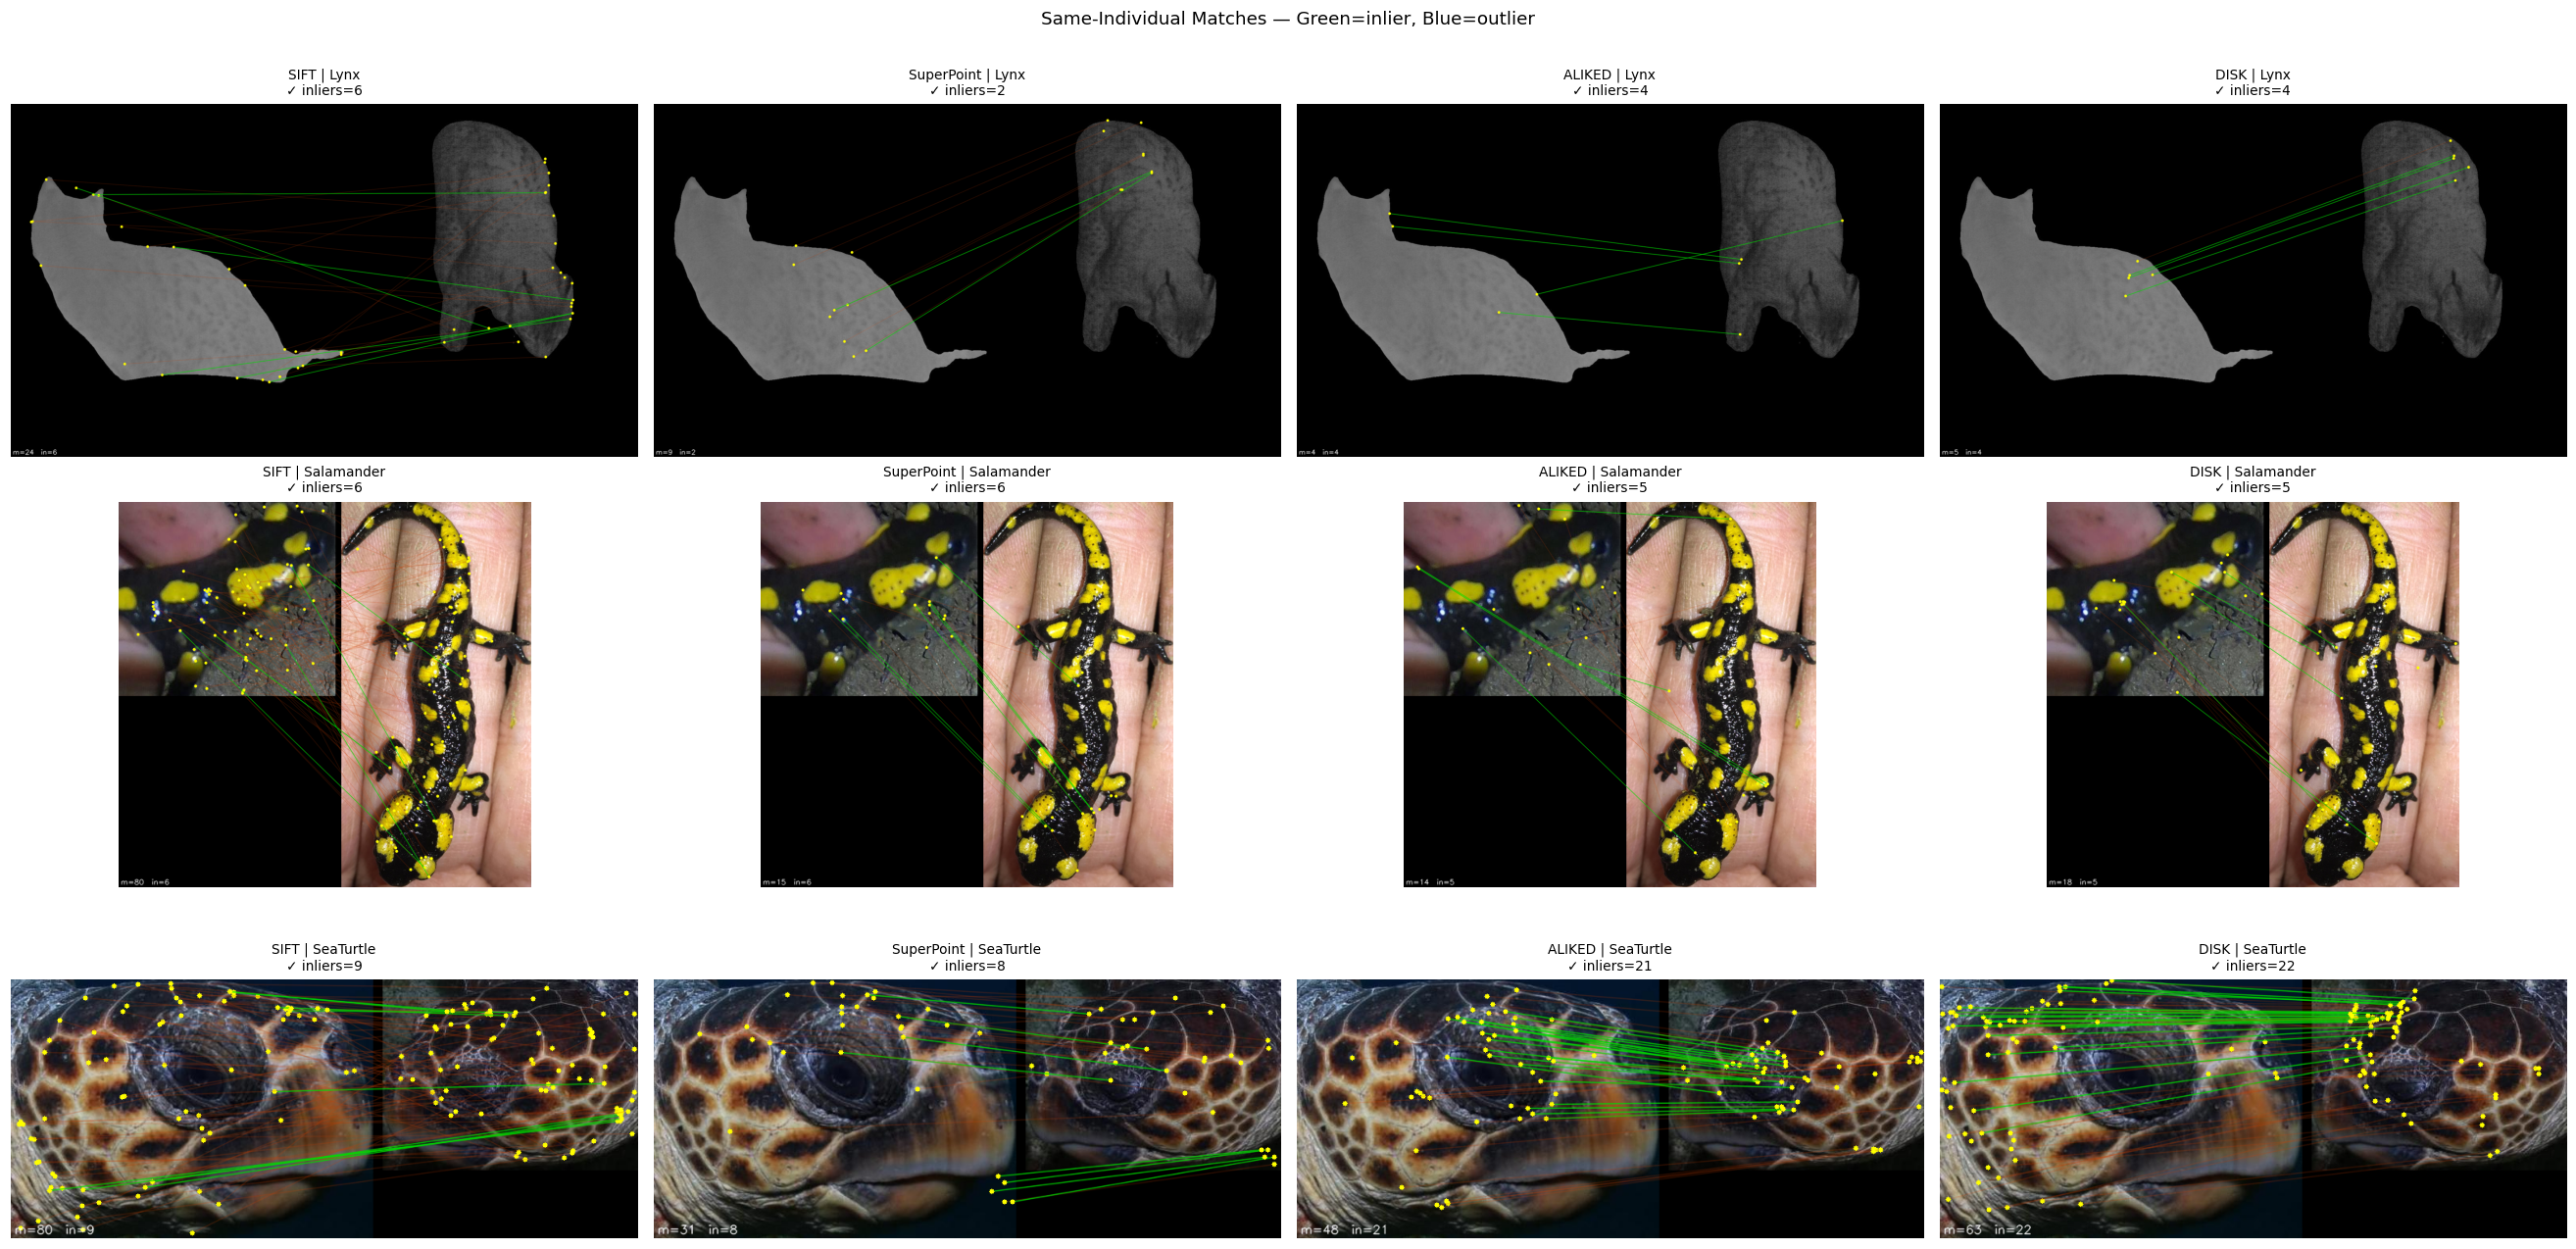
\includegraphics[width=\linewidth]{same_individual.png}
  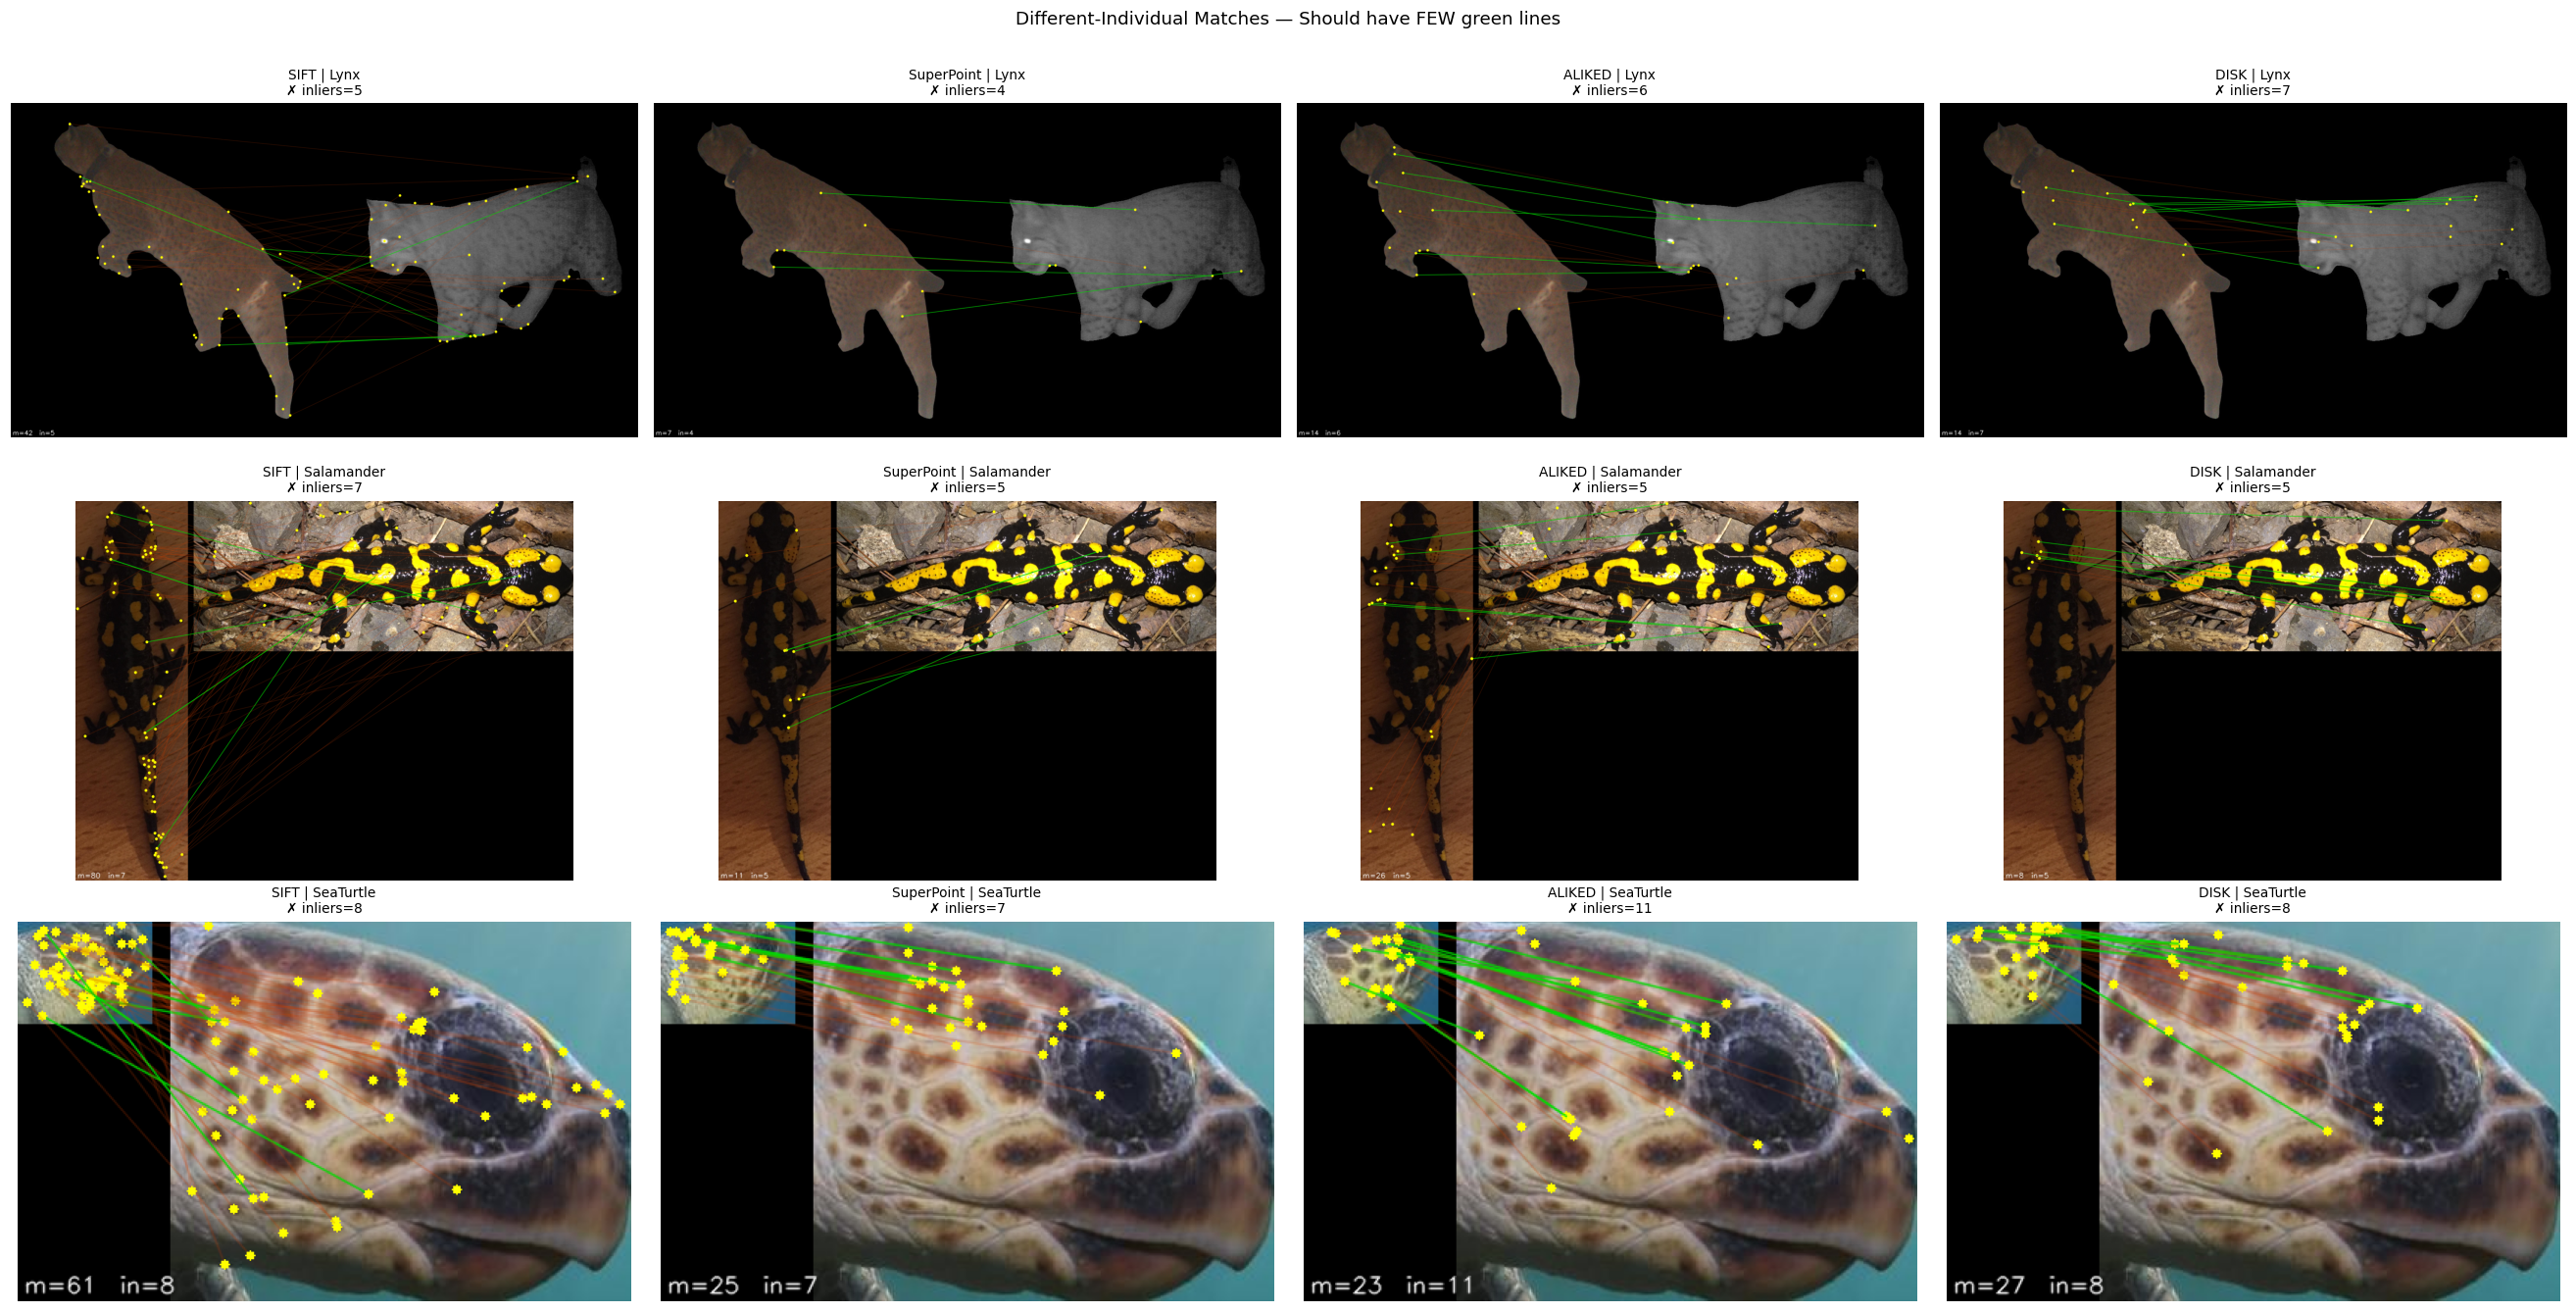
\includegraphics[width=\linewidth]{diff_individual.png}
  \caption{Top: keypoint matches for a same-individual pair --- dense and
    geometrically consistent. Bottom: a different-individual pair --- sparse and
    scattered. Match score is $1 - \exp(-n_\text{matches}/20)$.}
  \label{fig:matches}
\end{figure}

\textbf{SIFT + RootSIFT.} Standard SIFT followed by the RootSIFT
transform~\cite{arandjelovic2012three}: L1-normalize descriptors then take
element-wise square root. This converts L2 distance to Hellinger distance and
was a free +12.5\% improvement (V2.2). One gotcha: do not apply RootSIFT to
KAZE. KAZE descriptors are signed and the square root of negative values gives
NaN, silently zeroing all matches.

\textbf{KAZE.} Non-linear scale-space detector with 64-dim M-SURF descriptors.
Better than SIFT for dense biological texture because its anisotropic diffusion
scale space finds stable keypoints where SIFT's Gaussian pyramid just blurs
everything together. Added +7\% across V2.3b through V2.5.

\textbf{ALIKED + LightGlue.} ALIKED-n16~\cite{zhao2023aliked} paired with the
LightGlue GNN matcher~\cite{lindenberger2023lightglue}. Most useful for Lynx
(weight 0.35), which has zero SAM3 coverage --- the camera-trap IR images that
make up LynxID2025 don't segment cleanly, so classical extractors are noisier
there. ALIKED+LightGlue handles this better than SIFT/KAZE alone.

\subsection{Threshold Calibration}

For each species with training data, we grid-search over ensemble weights and
the clustering threshold, maximizing AMI against ground-truth labels. We
specifically do not use ARI here even though that is the competition metric.
The reason: ARI rewards large clusters and pushes thresholds too high, causing
systematic over-merging. When we tried ARI calibration (V4.0-ARI), Lynx
collapsed to 8 clusters from 946 images. AMI penalizes impure clusters so it
finds much better thresholds.

%% ─────────────────────────────────────────────────────────────────────────────
\section{Experiments}
%% ─────────────────────────────────────────────────────────────────────────────

\subsection{Data}

\begin{table}[h]
  \centering
  \caption{Per-species training data and the main challenge.}
  \label{tab:data}
  \begin{tabular}{lrrl}
    \toprule
    \textbf{Species} & \textbf{Train imgs} & \textbf{IDs} & \textbf{Challenge} \\
    \midrule
    LynxID2025         & 2,957 & 76  & IR images, no segmentation \\
    SalamanderID2025   & 1,388 & 587 & Too few images to fine-tune \\
    SeaTurtleID2022    & 8,729 & 412 & High viewpoint variation \\
    TexasHornedLizards & 0     & --- & Fully zero-shot \\
    \bottomrule
  \end{tabular}
\end{table}

\subsection{Ablation}

Table~\ref{tab:ablation} shows the score after each main change. Every row is
one actual Kaggle submission.

\begin{table}[h]
  \centering
  \caption{Score progression. Each version adds one change to the previous best.}
  \label{tab:ablation}
  \begin{tabular}{llr}
    \toprule
    \textbf{Version} & \textbf{Change} & \textbf{ARI} \\
    \midrule
    V1     & MiewID v3 + SIFT + BFMatcher     & 0.307 \\
    V1.3   & SAM3 keypoint mask filtering      & 0.325 \\
    V2.2   & +RootSIFT                         & 0.366 \\
    V2.3c  & +KAZE (THL and SeaTurtle)         & 0.377 \\
    V2.5   & +KAZE all species + AMI calib.    & 0.447 \\
    V2.8   & +Salamander yellow-spot ROI mask  & 0.462 \\
    V3.2.2 & +ALIKED+LightGlue, threshold fix  & 0.479 \\
    V4.0   & +Pretrained MegaDescriptor-L-384  & 0.486 \\
    V5.1   & +Fine-tuned MegaDescriptor-T-224  & \textbf{0.517} \\
    \bottomrule
  \end{tabular}
\end{table}

Figure~\ref{fig:ablation} visualizes the same progression.

\begin{figure}[h]
  \centering
  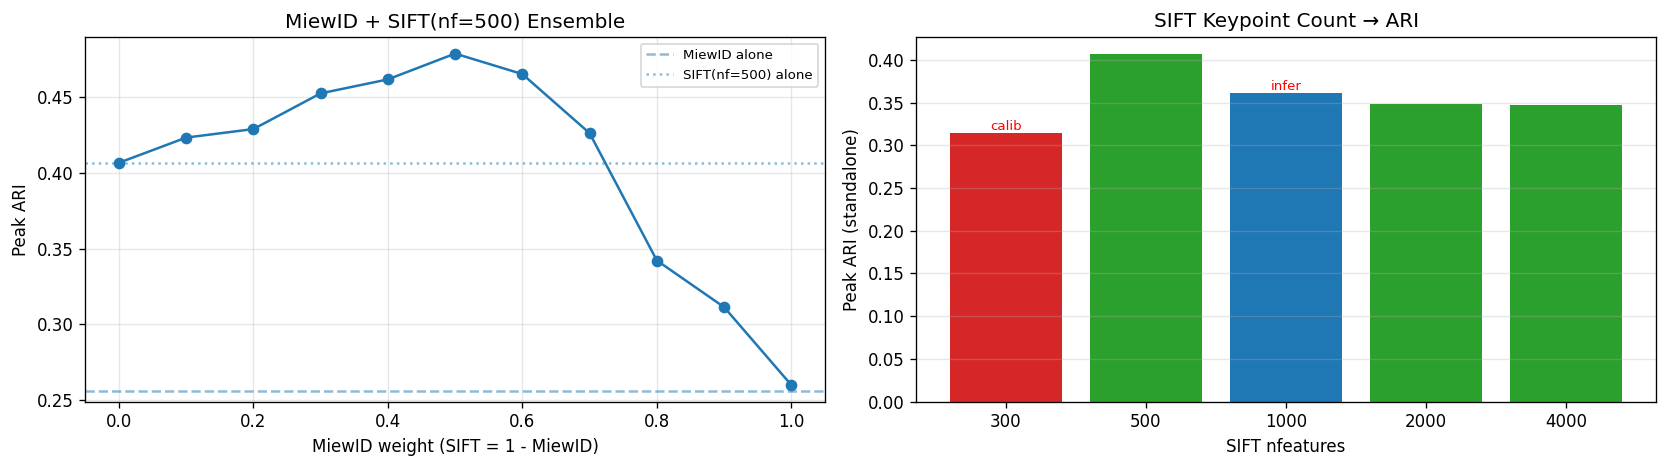
\includegraphics[width=\linewidth]{ablation.png}
  \caption{ARI score across submitted versions. Each bar represents a single
    submission. The biggest single jump (+0.07) came from adding AMI threshold
    calibration in V2.5.}
  \label{fig:ablation}
\end{figure}

\textbf{Fine-tuning impact by species.} The Lynx result is the most striking.
Pretrained MegaDescriptor was essentially useless for Lynx (weight 0.00 in V4.0
calibration), but after fine-tuning on CzechLynx it became the dominant feature
(weight 0.50 in V5.1). Training AMI went from 0.26 to 0.66. The CzechLynx
dataset~\cite{picek2025czechlynx} with 42k images was critical --- fine-tuning
on only the 2,957 competition Lynx images would not have been enough. For
SeaTurtle the fine-tuned model helped modestly. For Salamander, the fine-tuned
model got weight 0.00 in calibration, meaning it was actively ignored.

Figure~\ref{fig:heatmap} shows the per-extractor similarity heatmap for Lynx.
Each row/column is a test image; bright cells indicate high similarity. After
fine-tuning, the block-diagonal structure (same individual = high similarity)
is much cleaner.

\begin{figure}[h]
  \centering
  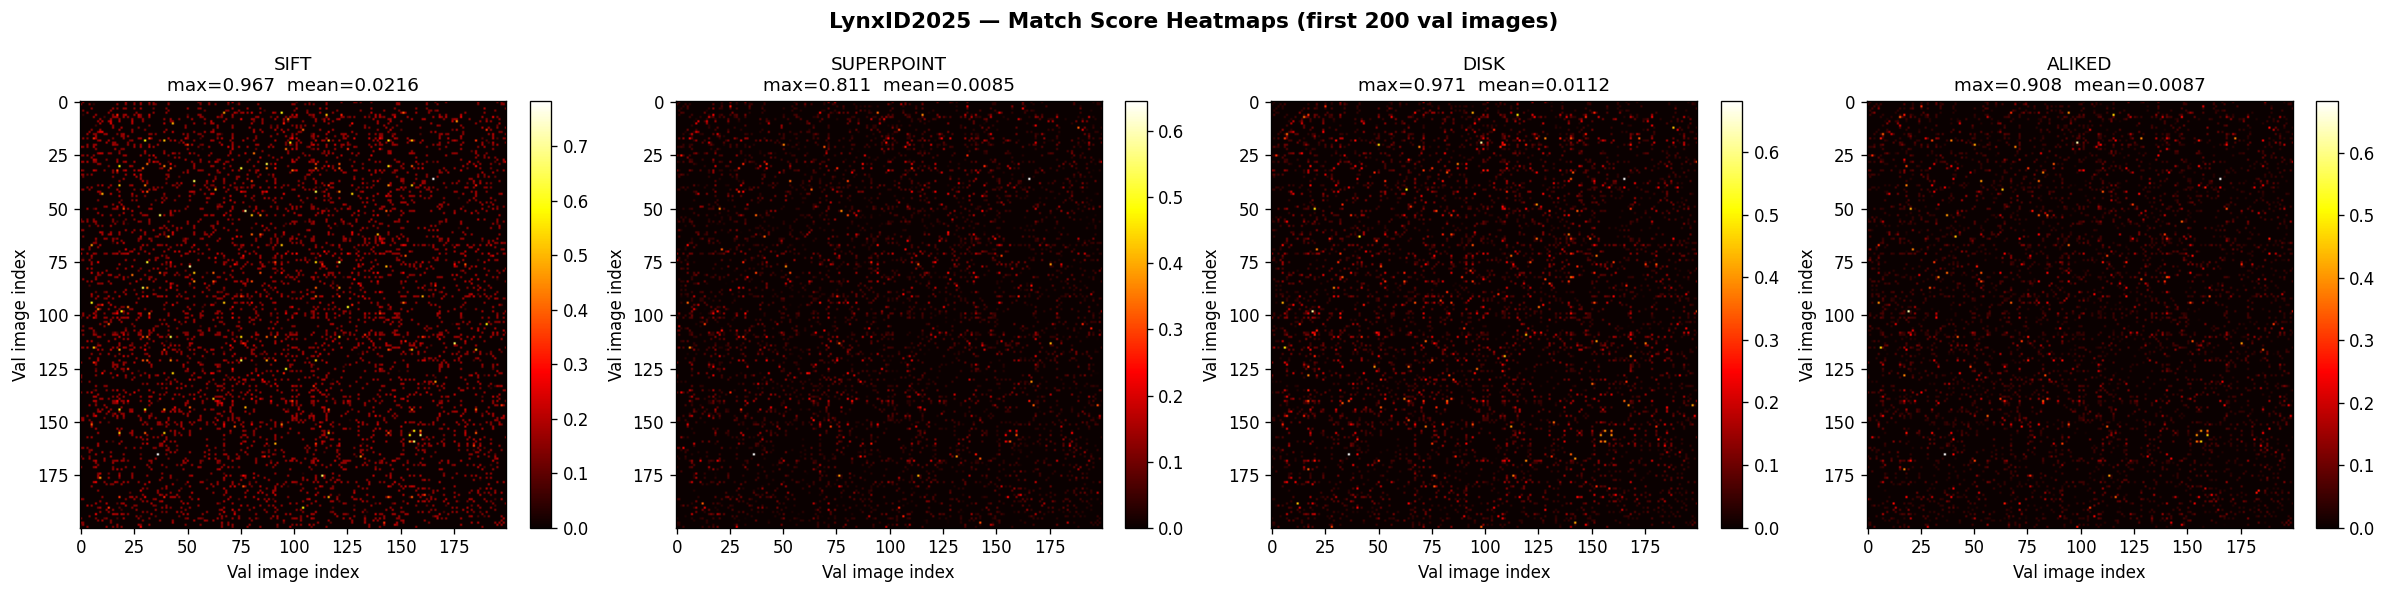
\includegraphics[width=\linewidth]{lynx_heatmap.png}
  \caption{Similarity heatmap for LynxID2025 test images. Rows/columns are
    sorted by ground-truth identity. Clear block-diagonal pattern means the
    model separates individuals well.}
  \label{fig:heatmap}
\end{figure}

\textbf{Final calibrated weights (V5.1):}

\begin{table}[h]
  \centering
  \caption{Per-species calibrated weights and clustering thresholds.}
  \label{tab:weights}
  \begin{tabular}{lrrrrrr}
    \toprule
    \textbf{Species} & \textbf{MiewID} & \textbf{MegaDesc} & \textbf{SIFT} & \textbf{KAZE} & \textbf{ALIKED} & \textbf{Thr.} \\
    \midrule
    Lynx       & 0.10  & 0.50  & 0.05 & 0.00 & 0.35 & 0.57 \\
    Salamander & 0.40  & 0.00  & 0.40 & 0.15 & 0.05 & 0.51 \\
    SeaTurtle  & 0.50  & 0.20  & 0.15 & 0.10 & 0.05 & 0.63 \\
    THL        & 0.275 & 0.275 & 0.15 & 0.10 & 0.20 & 0.30 \\
    \bottomrule
  \end{tabular}
\end{table}

%% ─────────────────────────────────────────────────────────────────────────────
\section{What Didn't Work}
\label{sec:failures}
%% ─────────────────────────────────────────────────────────────────────────────

These regressions cost us time but might save someone else's.

\textbf{LNBNN scoring (V2.0, ARI 0.107).} We tried replacing BFMatcher with
Local Naive Bayes Nearest Neighbor scoring, which is what HotSpotter uses. It
completely collapsed the score. The problem is the $K=100$ candidate preselection
--- the background pool ends up containing $\sim$100k descriptors from similar-looking
animals of the same species, so the ``background'' distance is nearly identical to
the match distance for almost every descriptor. Nearly all LNBNN deltas end up at
zero or negative, producing match scores that are effectively zero, and the ensemble
falls back entirely to the global cosine similarity with badly miscalibrated thresholds.
This is a known limitation of LNBNN in retrieval settings with a curated candidate set
rather than a large diverse database.

\textbf{Alpha Query Expansion (V2.4, ARI 0.356).} AQE on MiewID embeddings dropped
5.6\%. Intuitively it should help by pulling same-individual embeddings closer, but
in practice it did the opposite --- Salamander lost 105 clusters (different
individuals merged together) and Lynx gained 71 (same individuals split apart).
MiewID embeddings are already near their optimal configuration for this task;
smoothing them further just destroys the fine-grained structure. We checked the
per-pair agreement with V2.3c and it was 99.2--100\%, meaning the changes were real
but in the wrong direction.

\textbf{SuperPoint + LightGlue (V3.3, ARI 0.472).} Adding SuperPoint as a fourth
local extractor regressed from V3.2.2 (0.479). SuperPoint finds corners and junctions
--- features defined by image structure, not animal identity. A salamander's head
corner looks like every other salamander's head corner. The calibration correctly
assigned SuperPoint weight $= 0$ for Lynx, but just having it in the weight grid
shifted the thresholds for other species in a way that hurt.

\textbf{Fine-tuning MegaDescriptor-L-384 (V5.2--V5.4).} We tried upgrading from
T-224 (Swin-T, 28M params, 768-dim) to L-384 (Swin-L, 197M params, 1536-dim). Two
attempts, two failures. The first (V5.2) was too conservative: LR $3\text{e-}5$,
3 epochs for Lynx --- the model barely moved. The second (V5.4) was more aggressive
with LLRD and LR $1\text{e-}3$ and produced genuinely good embedding-space AMI
(+0.42 for Lynx, +0.33 for Salamander over pretrained), but regressed on the
leaderboard. The culprit was the expanded calibration grid --- we opened MegaDesc
weight up to 0.80, which overfit to training distribution. Lynx ended up with 18
clusters on the test set instead of the expected $\sim$40. The lesson here is boring
but real: don't expand calibration grids during a final sprint. Fix them once and
leave them.

\textbf{Isotonic score calibration (V5.0, ARI 0.348).} We tried isotonic regression
to normalize ensemble similarity scores to $[0,1]$ before thresholding. It compressed
all score distributions identically, which meant every species hit the 0.75 threshold
ceiling simultaneously. Salamander went from 492 clusters to a number much too low.
The issue is that isotonic calibration fitted to training score distributions does not
transfer to test score distributions when embeddings are as domain-dependent as they
are here. Removing it (V5.1) immediately recovered 0.17 ARI.

%% ─────────────────────────────────────────────────────────────────────────────
\section{Conclusion}
%% ─────────────────────────────────────────────────────────────────────────────

Our final submission (ARI 0.517 public, 0.471 private) uses MiewID v3 (frozen) plus
a fine-tuned MegaDescriptor-T-224, with RootSIFT, KAZE, and ALIKED+LightGlue on top,
all calibrated per species using AMI grid-search. A few things we are fairly confident
about after this competition: (1) For species with large external datasets, ArcFace
fine-tuning is worth doing --- CzechLynx took us from 0.486 to 0.517. (2) Use AMI
for threshold calibration, not ARI. (3) KAZE is better than SIFT for animals with
dense texture patterns. (4) Use segmentation masks to filter keypoints after extraction,
not to pre-process images before it. (5) Salamander is hard and we don't have a good
answer for it --- 1,388 images for 587 identities is just not enough for fine-tuning,
and there is no large-scale public fire salamander re-ID dataset to help.

%% ─────────────────────────────────────────────────────────────────────────────
\bibliography{sample-ceur}
%% ─────────────────────────────────────────────────────────────────────────────

\end{document}
